\section{Conception et développement}

\begin{frame}
\tableofcontents[currentsection]
\end{frame}

\begin{frame}
	\frametitle{Conception base de données}
	Comment stocker correctement les questions/réponses ?
	
	\begin{figure}[!h]
		\centering
			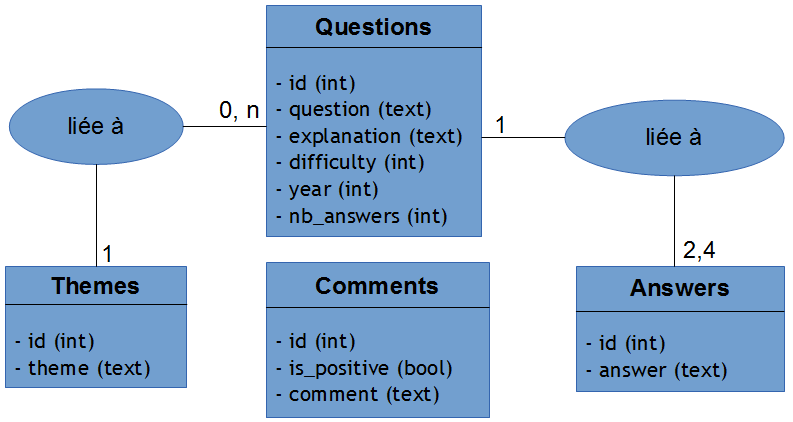
\includegraphics[width = 0.9\textwidth]{conception/bdd.png}
		\label{Schéma base de données} 
		\caption{Schéma base de données}
	\end{figure}
\end{frame}

\begin{frame}
	\frametitle{Conception base de données}
	Discussion du modèle utilisé : dépend des critères recherchés
		
	\bigskip

	\begin{columns}[t]
		\begin{column}{10cm}
			\begin{exampleblock}{Notre architecture}
				\begin{itemize}
					\item[-] est plus complexe au premier abord
					\item[-] nécessite un peu d'algorithmique
				\end{itemize}
			\end{exampleblock} 
		\end{column}
	\end{columns}
	
	\begin{columns}[t]
		\begin{column}{10cm}
			\begin{exampleblock}{Mais au final}
				\begin{itemize}
					\item[+] l'évolution et la maintenance sont facilitées
				\end{itemize}
			\end{exampleblock} 
		\end{column}
	\end{columns}
\end{frame}

\begin{frame}
	\frametitle{Architecture de classes}
	Calquée sur un modèle MVC (Modèle, Vue, Contrôleur)
	
	\begin{figure}[!h]
		\centering
			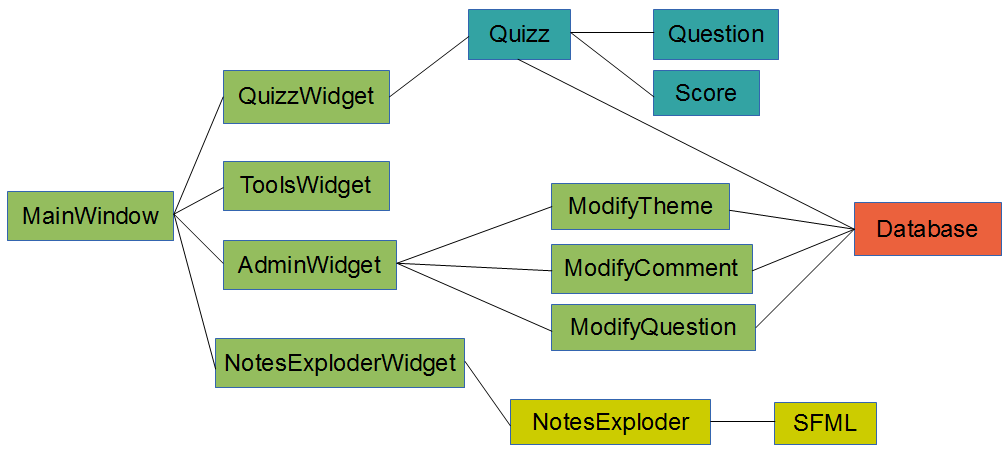
\includegraphics[width = 0.9\textwidth]{conception/classes.png}
		\label{Schéma des classes} 
		\caption{Schéma des classes}
	\end{figure}
\end{frame}

\begin{frame}
	\frametitle{Développement}
	Le modèle MVC nous a facilité le développement
		
	\begin{columns}[t]
		\begin{column}{10cm}
			\begin{exampleblock}{Avantages de MVC}
				\begin{itemize}
					\item[+] répartition du travail en équipes de deux
					\item[+] chaque groupe est indépendant
					\item[+] chaque module offre des services aux autres
				\end{itemize}
			\end{exampleblock} 
		\end{column}
	\end{columns}
	
	\bigskip
	
	Nécessite une conception rigoureuse en amont afin de pouvoir tout fusionner
	sans problème à la fin!
\end{frame}

\begin{frame}
	\frametitle{Développement}
	Les technologies utilisées sont inter-compatibles.
		
	\begin{columns}[t]
		\begin{column}{10cm}
			\begin{exampleblock}{Technologies utilisées}
				\begin{itemize}
					\item Langage de base : C++ orienté objet
					\item Qt : C++ orienté objet
					\item SFML : C++ orienté objet
				\end{itemize}
			\end{exampleblock} 
		\end{column}
	\end{columns}
	
	\bigskip
	
	=> Code homogène et découpage en classes intuitif
\end{frame}